\section{Introduction}\label{sec:intro}
The ubiquity of location acquisition devices leads to an explosive growth of movement data (i.e., trajectories), e.g., for vehicles, shared bikes and pedestrians. Visualizing these large-scale trajectory data is crucial for many smart city applications~\cite{wang2014visual, tang2017efficient, zheng2011learning, zeng2014visualizing} and location-based services~\cite{liu2016smartadp, zheng2010collaborative}. Among various visualization methods, line-based trajectory visualization, which connects the locations of a moving object by polylines, is widely adopted for spatial-temporal data analytics~\cite{chen2015survey, visualanalysis, bigchanvis}. To support interactive exploration on trajectory data, it is crucial to conduct line-based trajectory visualization for an arbitrary region with high quality and low latency.

%\stitle{Long visualization time for large-scale datasets}
\stitle{Challenge for visualizing full datasets} To visualize the trajectories in a target region $\query$, a natural solution is to find the trajectories in it and visualize all these trajectories ($\full$ for short). However, $\full$ may suffer from a long visualization time as the trajectory datasets can be extremely large. For example, Shenzhen has 24,237 taxis which collectively generate more than 7.72 million GPS locations each day~\cite{sz}. Our profiling results in Table~\ref{tab:gpu}\footnote{Mapping is the time to map the GPS points to the screen points, and rendering is the time to render the graphics. The details can be found in Section~\ref{sec:exp}.} also show that visualizing the 1,000,000 taxi trajectories needs 16.154 seconds which is far more than 2 seconds delay suggested for interactive exploration~\cite{shneiderman1984response}.
%However, interactive visual exploration typically requires the visualization to be generated in less than 1 second~\cite{shneiderman1984response}. 
Another problem of applying $\full$ on large-scale datasets is~\textit{visual clutter}~\cite{kwon2017sampling}, where there are too many points in the visualization such that it is difficult for users to gain insights. One such example can be found in Figure~\ref{fig:overview}(A), for which it is difficult to recognize the road networks in the dense center region.   


%We provide an example Figure~\ref{fig:overview}(A) for the \pt{} dataset, for which it is almost impossible to recognize the road networks in the dense region at the center.

\begin{table}
	\centering
	\small
	\caption{Visualization time on the \pt{} dataset (in seconds)}
	\vspace{-2mm}
    \trim
	\begin{tabular}{|c|c|c|c|c|} \hline
		No. of  & No. of & Mapping & Rendering & Total \\
         trajectories &  GPS points & time & time & time \\ \hline
		1,000& 31,300 & 0.027 & 0.003 & 0.03 \\ \hline
		10,000& 31,6531 & 0.169 & 0.005 & 0.174\\ \hline
		100,000& 316,7120 & 1.701 & 0.057 & 1.758 \\ \hline
		1,000,000& 31,646,379 & 15.562 & 0.592 & 16.154 \\ \hline
	\end{tabular}	\label{tab:gpu}
    \trim \trim 
\end{table}

\if 0
\begin{figure*}[t]
	\centering
	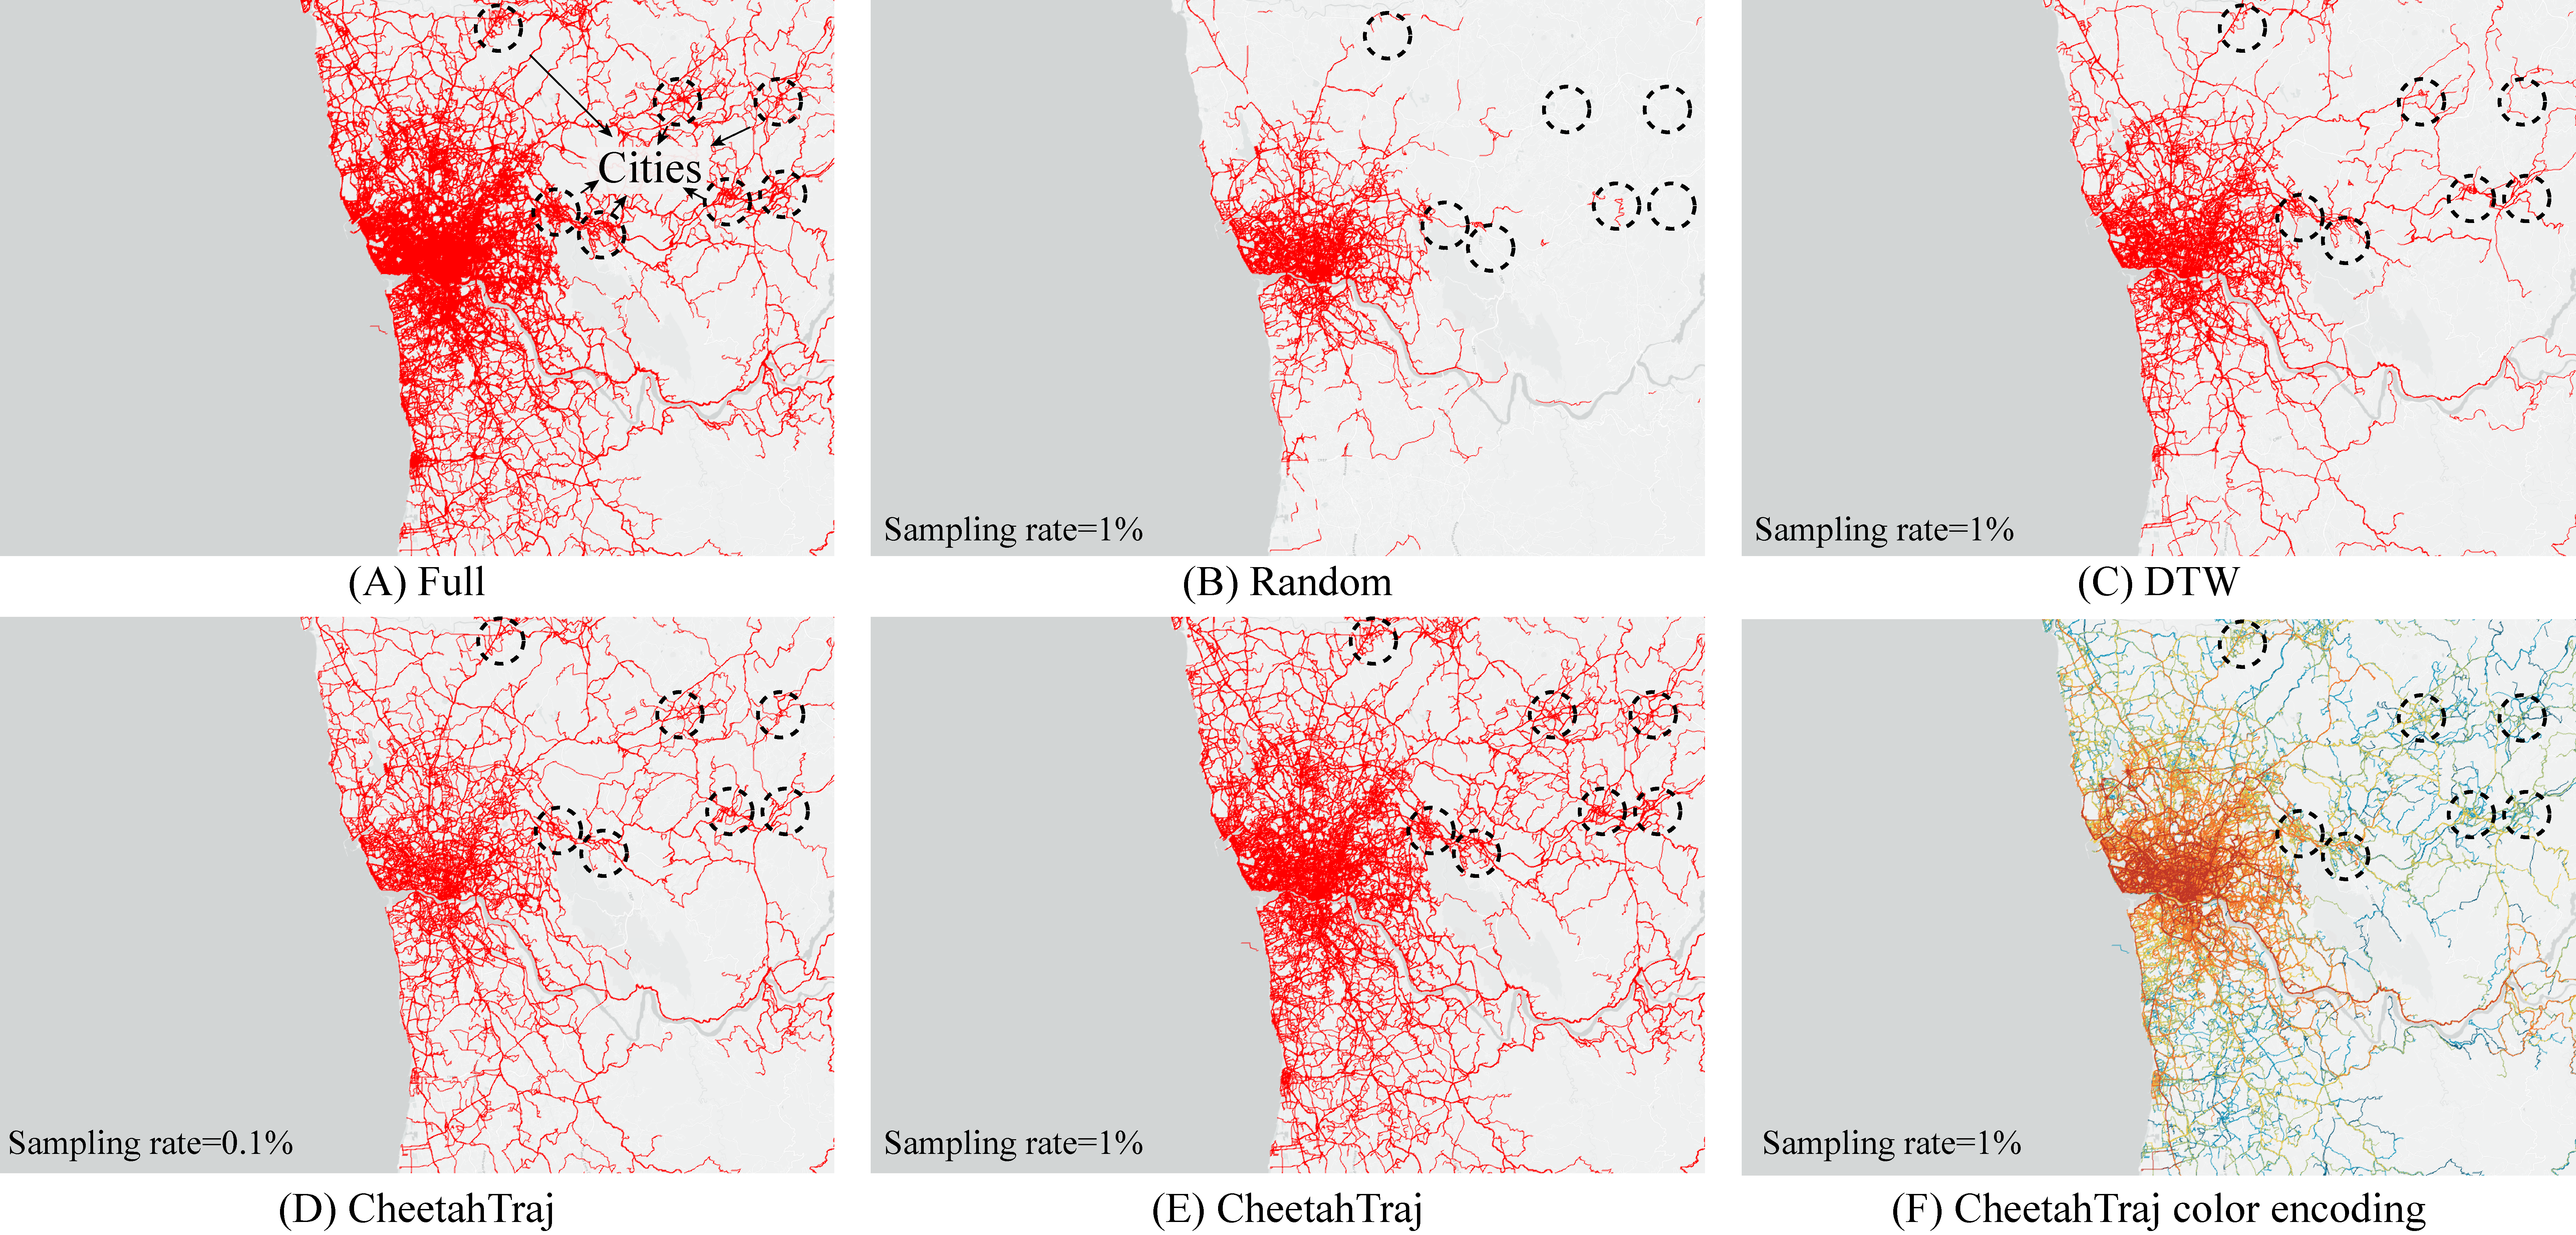
\includegraphics[width=0.75\textwidth]{pictures/case_study_icde/case_study_overview.pdf}
	\trim
	\caption{Effectiveness of $\avats$ at overview visualization in \pt{}.}
	\label{fig:overview}
	\trim \trim
\end{figure*}
\fi
%\stitle{Ad-hoc sampling has poor visual quality} Sampling techniques are widely used to accelerate large-scale data analysis in both database and visualization communities~\cite{qin2020making,DBLP:conf/sigmod/DingHCC016,DBLP:journals/pvldb/KimBPIMR15,park2016visualization}. By selecting a subset of the trajectories in the target region for visualization, sampling can reduce both visualization time and visual clutter. One such example is ScalaR~\cite{battle2013dynamic}, which employs a reduction layer between the visualization layer and the data management layer. The reduction layer samples records \textit{uniformly at random} (denoted as $\rand$) when the query results are too large. However, $\rand$ has poor visual quality as its visualization could be significantly different from the ground-truth. We provide such an example in Figure~\ref{fig:overview}(B), where $\rand$ fails to include trajectories in the sparse areas of Figure~\ref{fig:overview}(A). Another natural idea is to sample trajectories with good diversity and we develop such a baseline using the famous Dynamic Time Warping (DTW) distance between trajectories~\cite{borcan2012improving}. As shown in Figure~\ref{fig:overview}(C), $\mathsf{DTW}$ provides better visualization than $\rand$ but there are still obvious differences between $\mathsf{DTW}$ and the ground-truth in Figure~\ref{fig:overview}(A). Without explicit visual quality guarantee, sampling trajectories in ad-hoc ways may produce visualizations with poor quality and mislead visual exploration.

\stitle{Ad-hoc sampling has poor visual quality} Sampling is widely used to accelerate large-scale data analysis in both information retrieval and data visualization~\cite{qin2020making,DBLP:conf/sigmod/DingHCC016,DBLP:journals/pvldb/KimBPIMR15,park2016visualization}. 
% By selecting a subset of the trajectories in the target region for visualization, sampling can reduce both visualization time and visual clutter. 
One such example is ScalaR~\cite{battle2013dynamic}, which samples records \textit{uniformly at random} (denoted as $\rand$) when the query results are too large. However, $\rand$ has poor visual quality as its visualization can be significantly different from the ground-truth in the sparse areas as shown in Figure~\ref{fig:overview}(B). 
%As shown by Figure~\ref{fig:overview}(B), where $\rand$ fails to include trajectories in the sparse areas of Figure~\ref{fig:overview}(A). 
Another natural idea is to sample trajectories with good diversity and we develop such a baseline using the famous Dynamic Time Warping (DTW) distance between trajectories~\cite{borcan2012improving}. As shown in Figure~\ref{fig:overview}(C), $\mathsf{DTW}$ provides better visualization than $\rand$ but there are still obvious differences between $\mathsf{DTW}$ and the ground-truth in Figure~\ref{fig:overview}(A). 
Without explicit visual quality guarantee, sampling trajectories in ad-hoc ways may produce visualizations with poor quality and mislead visual exploration.


\stitle{The $\avats$ framework} We explore novel algorithm and efficient index jointly in the $\avats$ framework to provide visualizations with high quality and low latency. To conduct quality guaranteed sampling, we first propose a novel pixel-based \textit{visual quality function} to measure how similar an approximate visualization is to the ground-truth. We also show that it is NP-hard to select an optimal set of trajectories that maximize the visual quality function. Next, we devise a \textit{visual quality guaranteed sampling algorithm} named $\vats$, which provides theoretical visual quality guarantee for the sampled trajectories. Then, we \textit{tackle the visual clutter problem} by taking data distribution and human perception into consideration in an advance algorithm named $\vatss$. To avoid running the somehow complex $\vatss$ algorithm on-line for interactive visual exploration, we design an $\invQ$-tree index based on quad-tree, which allows to use the sampling results computed in an offline index building phase. 

%We conducted extensive case study, user study and quantitative performance evaluation to show the effectiveness of $\avats$.

%

%$\invQ$-tree allows to directly use the sampling results computed in an offline index building phase and provides quality guaranteed trajectory samples for an arbitrary target region.

We conduct extensive case study, user study and quantitative performance evaluation to validate the visualization quality and efficiency of the $\avats$ framework. The case study shows that $\avats$ consistently provides high quality visualizations for both large target regions and small target regions. The user study with 35 participants confirms that $\avats$ effectively reduces visual clutter and produces visualizations that are plausible to human inspectors. The quantitative performance evaluation shows that $\avats$ provides good visual quality by sampling only a small number of trajectories. In addition,  $\avats$ produces high quality visualizations for arbitrary target regions in less than 1 second for all 3 experiment datasets and the visualization delay is below 0.1 second in most cases.


We illustrate the merits of our $\avats$ framework in Figure~\ref{fig:overview}. Figure~\ref{fig:overview}(D) and (E) are the visualizations produced by $\avats{}$ on the \pt{} dataset with sampling rate $0.1\%$ and $1\%$, respectively. Compared with uniform random sampling (i.e., $\rand$) and diversity based sampling (i.e., $\mathsf{DTW}$) in Figure~\ref{fig:overview}(B) and (C), Figure~\ref{fig:overview}(D) and (E) are obviously more similar to the full dataset visualization in Figure~\ref{fig:overview}(A).
Figure~\ref{fig:overview}(F) is produced by $\avats{}$ using the same parameters as Figure~\ref{fig:overview}(E) but the trajectories are colored according to their algorithm-generated representativeness (warmer color means more representative). Compared with Figure~\ref{fig:overview}(A), the main routes in the dense region can be identified much more easily, which shows that $\avats{}$ effectively reduces visual clutter. Last but not least, it takes $\avats{}$ only 0.116 seconds and 0.339 seconds to generate Figure~\ref{fig:overview}(D) and (E), respectively, while the full visualization in Figure~\ref{fig:overview}(A) takes 16.154 seconds.



%To sum up, our technical contributions in this paper include:
%
%\squishlist
%  \item We formulate the visual quality optimal trajectory sampling problem for large-scale trajectory data visualization, and prove that it is {NP-hard} (Section~\ref{sec:pro}).
%  \item We devise an approximate algorithm $\vats$ for the visual quality guaranteed sampling problem. $\vats$ is further improved with $\vatss$ by considering data distribution and human perception (Section~\ref{sec:sol}).
%  \item We propose the $\avats$ framework, which jointly uses the aforementioned algorithms and tailored index to achieve both quality and efficiency in large-scale trajectory data visualization (Section~\ref{sec:cheetahtraj}).
%
%\squishend
%
%
%
%This rest of the paper is organized as follows. Section~\ref{sec:rel} introduces related works. The quality optimal trajectory sampling problem is formulated and analyzed in Section~\ref{sec:pro}. Section~\ref{sec:sol} presents our $\vats$ and $\vatss$ algorithm for quality guaranteed trajectory sampling. Section~\ref{sec:cheetahtraj} elaborates the $\avats$ framework. The experiment results are presented in Section~\ref{sec:exp}. Section~\ref{sec:con} draws the conclusions.
